\documentclass[border=2pt,tikz]{standalone}
\usepackage{tikz}
\usepackage{amsmath}
\usepackage{amssymb}

\begin{document}

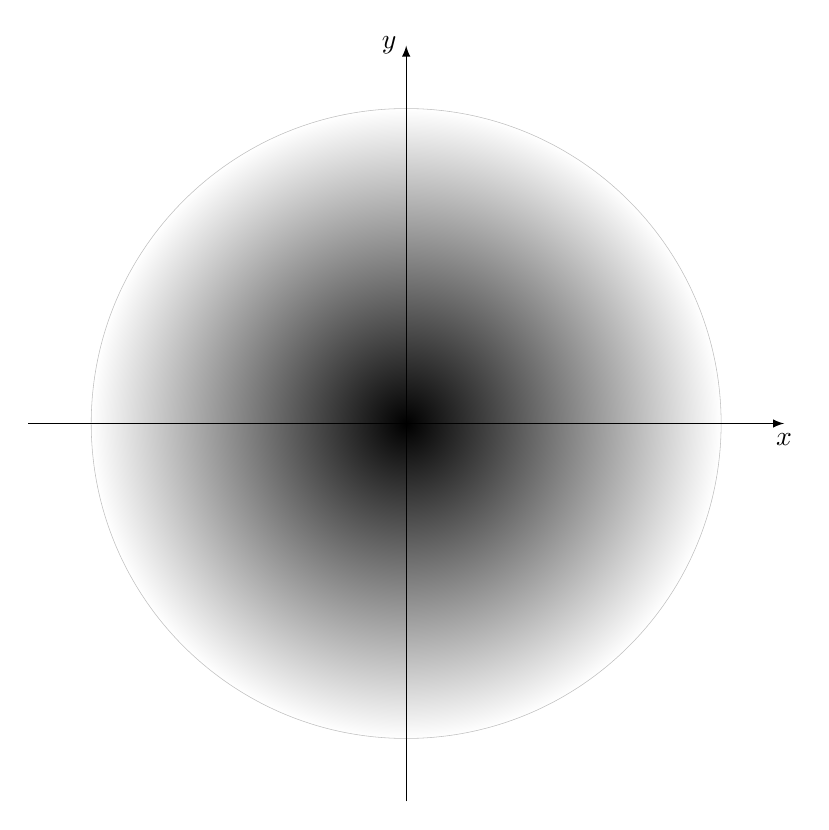
\begin{tikzpicture}[scale=4]

% Draw a circle at the origin of radius 1
\draw [very thin, lightgray, inner color=black!100, outer color=black!0] (0,0) circle (1);

% Draw x and y axis lines
\draw [->,>=latex] (-1.2,0) -- (1.2,0) node [below] {$x$};
\draw [->,>=latex] (0,-1.2) -- (0,1.2) node [left] {$y$};

\end{tikzpicture}

\end{document}

